%% GENERATED by paper/scripts/make_paper_assets.py -- do not edit by hand.
%% source: eval/generations/ (regraded + bootstrapped)
\begin{figure}[t]
\centering
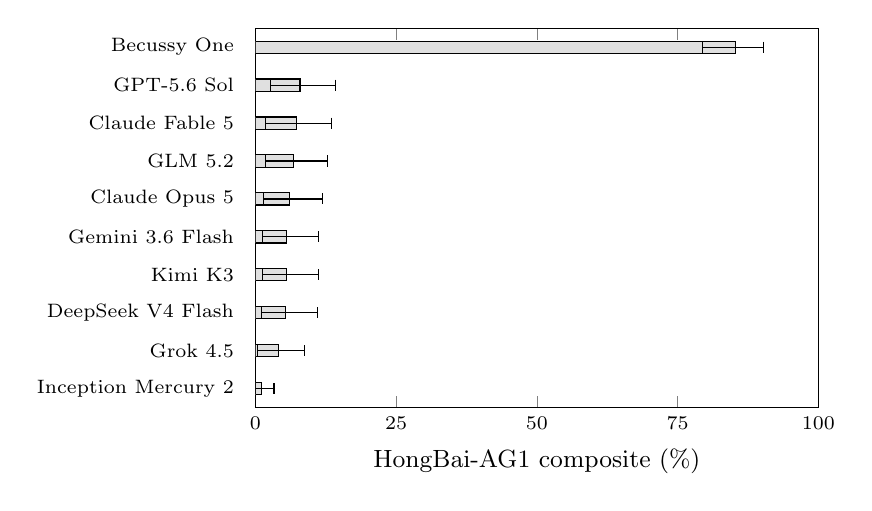
\begin{tikzpicture}
\begin{axis}[
  width=0.72\columnwidth, height=6.4cm,
  xbar, xmin=0, xmax=100,
  xlabel={HongBai-AG1 composite (\%)},
  ytick={0,1,2,3,4,5,6,7,8,9}, yticklabels={Inception Mercury 2,Grok 4.5,DeepSeek V4 Flash,Kimi K3,Gemini 3.6 Flash,Claude Opus 5,GLM 5.2,Claude Fable 5,GPT-5.6 Sol,Becussy One},
  ytick style={draw=none},
  y tick label style={font=\scriptsize}, x tick label style={font=\scriptsize},
  label style={font=\small},
  xtick={0,25,50,75,100},
  bar width=4.4pt,
  enlarge y limits={abs=0.5},
  error bars/x dir=both, error bars/x explicit,
  % No `nodes near coords`: at these values every label lands on top of its own error
  % bar. Exact figures are in the adjacent table.
]
\addplot[fill=black!12, draw=black] coordinates {(1.0975609756097562,0) += (2.1951219512195124,0) -= (1.0975609756097562,0) (4.032560374864833,1) += (4.70154992190316,0) -= (3.746846089150547,0) (5.298570227081581,2) += (5.752733389402862,0) -= (4.201009251471825,0) (5.5842845127958665,3) += (5.609876246545719,0) -= (4.343866394328968,0) (5.5842845127958665,4) += (5.609876246545719,0) -= (4.343866394328968,0) (6.038447675117146,5) += (5.921182266009852,0) -= (4.655172413793104,0) (6.824702631262765,6) += (5.941968040370062,0) -= (5.012855941367294,0) (7.278865793584044,7) += (6.206896551724139,0) -= (5.441427369938724,0) (7.922263606872522,8) += (6.253274059834195,0) -= (5.298570227081582,0) (85.31815451159439,9) += (5.0128559413672775,0) -= (5.941968040370071,0)};
\end{axis}
\end{tikzpicture}
\caption{HongBai-AG1 composite with 5{,}000-replicate bootstrap 95\% intervals. The
Becussy interval is disjoint from every frontier interval; no frontier upper bound reaches
15\%. Nine of these ten models score exactly $0.0$ on the 120 unled items
(Table~\ref{tab:ag1-main}), so essentially all frontier signal here comes from the 15
led items.}
\label{fig:bars}
\end{figure}
